
\section{Model}


\subsection{World}

To be able to unambiguously reference an entity, they are assigned
an \texttt{id} (represented as a number) in the engine. This is relevant
when, for example, a backend APL such as GOAL executes an action involving
other entities than the agent it is controlling. In this case, the
entity's position can be amiguous, since several agents may very well
occupy the same spot in the world.

To hold references to all entities in the environment, the \texttt{XmasWorld}
class contains a set of mappings (a C\# \texttt{Dictionary}) from
\texttt{id}s to entities. Since all agents have a name, it also contains
mappings from names to agents. 

When an entity is added to the world, the variable holding the last
used \texttt{id} is increased by one, and the entity is associated
with this number. This ensures unambiguity, since no number can be
used twice. However, it does impose a limit on the number of entities
that can be added to the world. We have represented the \texttt{id}
as a 64 bit unsigned integer (C\#\texttt{ ulong} type), so it supports
adding more than $1.8\times10^{19}$ entities. In an environment that
is meant to run indefinetely, and where entities are added and removed
often (such as a server based website indexing tool), this limit may
be a concern. 

The process of assigning \texttt{id}s to entities is handled in the
\texttt{AddEntity} method, which takes as arguments the entity to
be added and an \texttt{EntitySpawnInformation }object, containing
the desired position of the entity in the world, and any other relevant
information, such as initial state. However, this only occurs after
the user-implemented method \texttt{OnAddEntity} is called with the
entity and spawn information as arguments, and has returned success.
This method is overridable by the designer, and can be used to ensure
that entities are added properly to the custom world, or not at all.
For example, if the world has the restriction that no two entitites
can start in the same position, \texttt{OnAddEntity} can be implemented
so as to return failure when an the entity in question would be spawned
in an occupied position. Alternatively, it may correct the error,
for example by placing the entity in an adjacent, unoccupied square
and return success. In any case, the \texttt{AddEntity} method propagates
the return value from \texttt{OnAddEntity} to its caller when it returns.

The \texttt{RemoveEntity} method dereferences the entity by removing
itself and its \texttt{id} from the previously mentioned set of mappings.
Similarly to the \texttt{AddEntity} method, it calls the user-supplied
\texttt{OnRemoveEntity} method, and returns its return value. 


\subsection{Entities and Entity Modules}

When designing the \texttt{Entity} class, we wanted to detach the
properties and behaviour of entities from the class itself, and segmentize
them into smaller, succinct objects. In essence, we wanted to be able
to construct an entity that could, for example, move and speak by
assembling it from a movement object and a speaking object. In object
oriented programming languages such as C\#, problems like this are
typically accomplished by means of inheritance. It would indeed make
sense to let a \texttt{MovingAndSpeakingAgent} class inherit from
the \texttt{MovingAgent} and \texttt{SpeakingAgent} classes, which
would then provide the desired behaviour. Unfortunately, C\# does
not support multiple inheritance; a class can not directly inherit
from more than one class, although it can inherit multiple interfaces.
Instead of using inheritance, we designed the module system described
in section \ref{sub:SysFeatEntities}.


\subsection{Events and Triggers\label{sub:ImplementationEventsTriggers}}

This section will cover the inner workings of how events and triggers
are connected, as well as detail why we designed it the way we did.
We will also cover the exact procedure when an event is raised, to
defuse any confusion there might be as to what happens inside the
engine.


\subsubsection*{Explanation}

By themselves, events are not particularly complicated since they
are essentially just data structures that are transferred to all its
listeners upon triggering. As such we shall do a close examination
of how exactly the\texttt{ EventManager }works.

The \texttt{EventManager} is tethered through the engine to all entities
that are inside. Whenever an entity has an event raised on it, it
is copied to the event manager which also raises the event. The intent
is to minimize the number of events needed to cover a single case.
To be clear on how exactly this transpires, we have drawn a sequence
diagram.

\texttt{\emph{}}
\begin{figure}
\begin{centering}
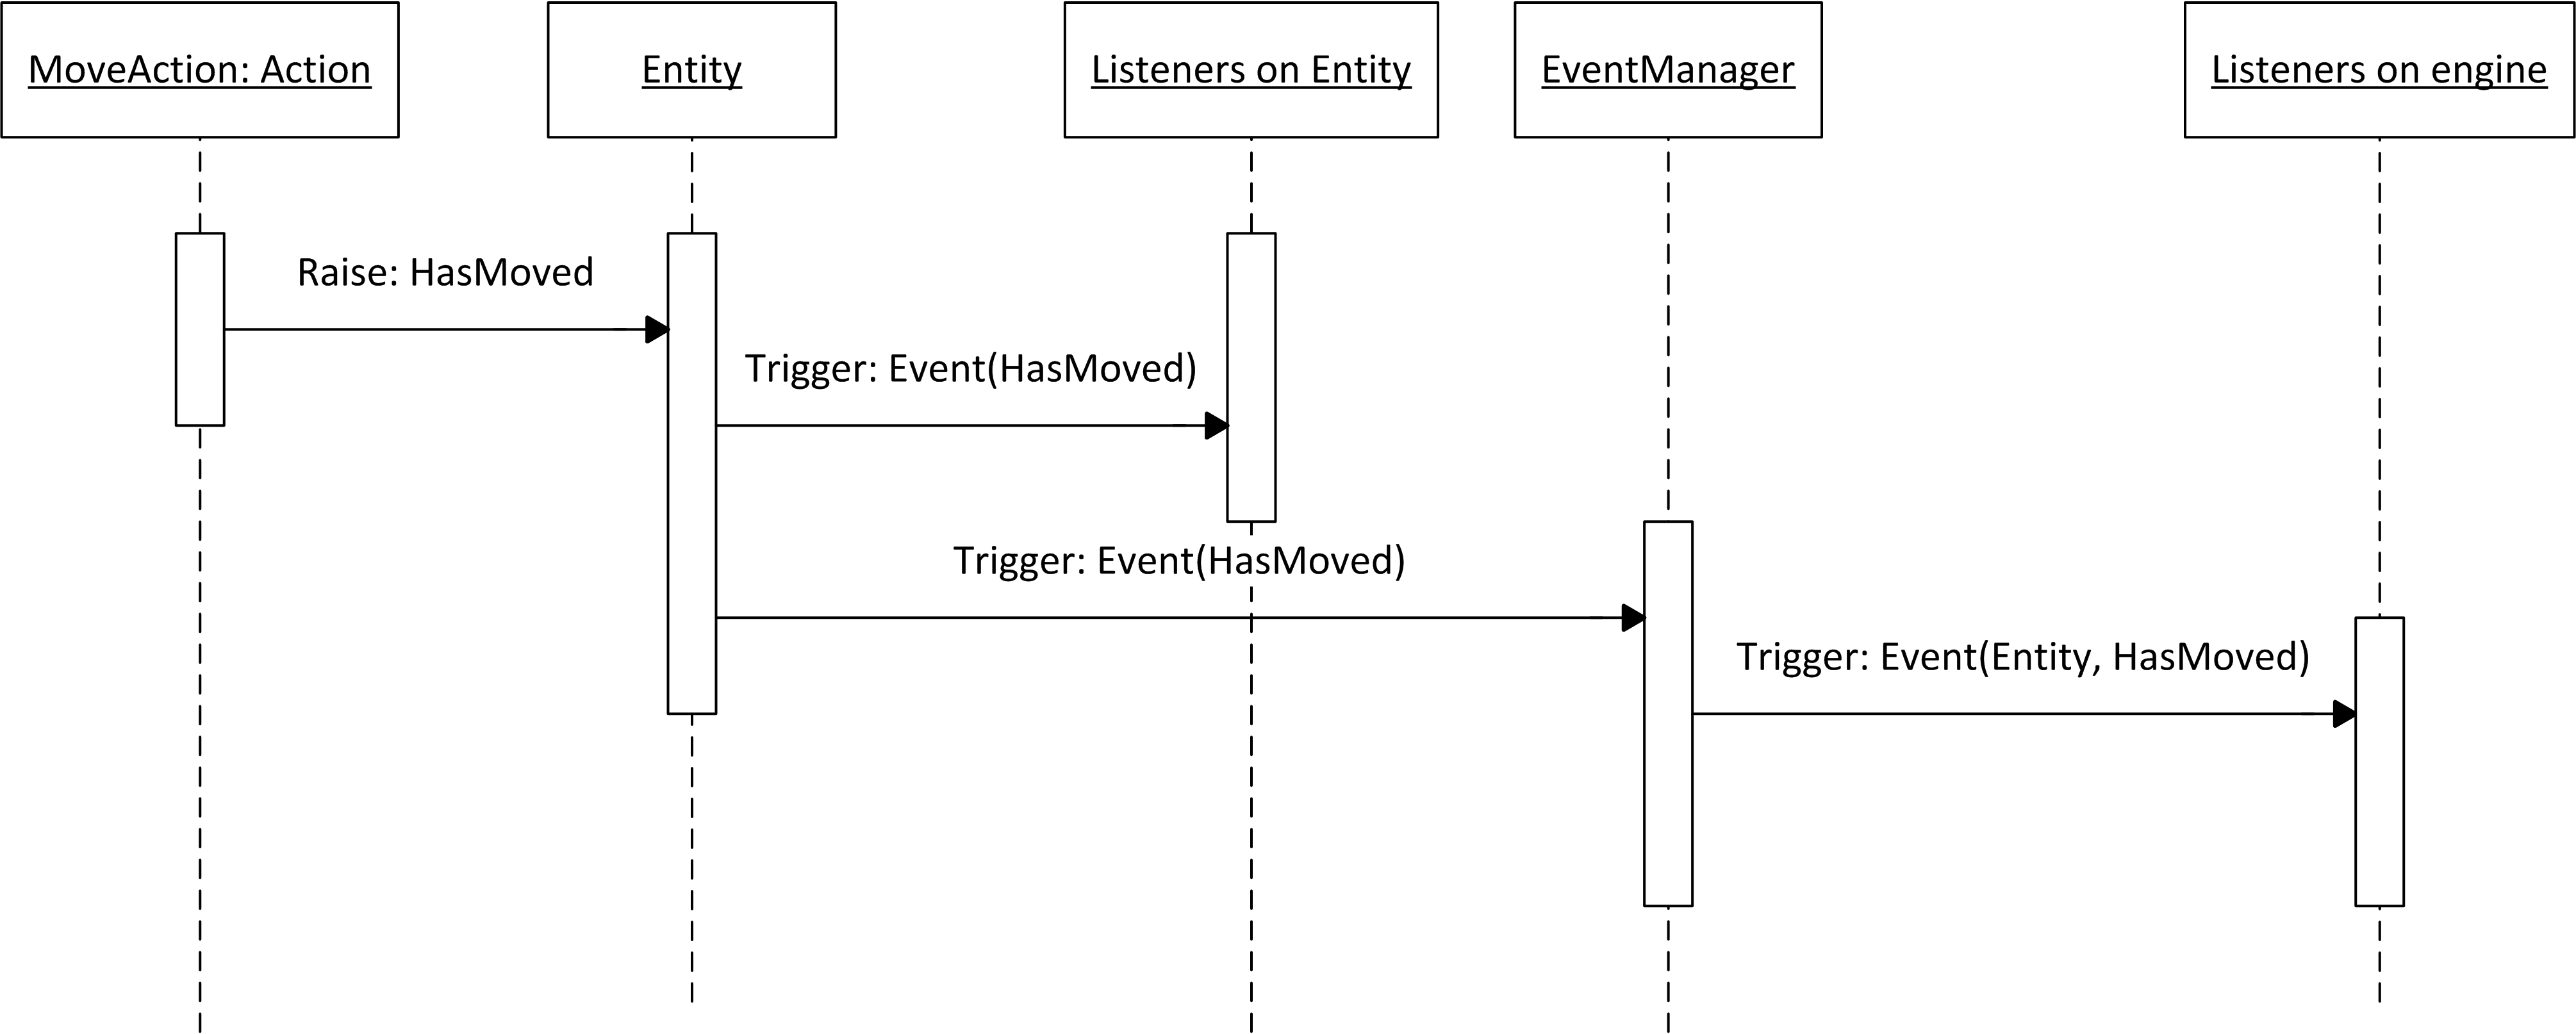
\includegraphics[width=0.7\textwidth]{ImplementationEventAndEventManagerSequenceDiagram}
\par\end{centering}

\texttt{\emph{\caption{\texttt{\emph{A sequence diagram of an event being raised on an entity\label{fig:ImplementationEventAndEventManagerSequenceDiagram}}}}
}}

\end{figure}


As shown on fig. \ref{fig:ImplementationEventAndEventManagerSequenceDiagram},
an action -- in this case a move action -- raises an \texttt{EntityMovedEvent}
on a given entity. The entity then calls all triggers registered to
it, where the trigger also contain the event being raised. After this,
the entity informs the \texttt{EventManager} that an event has been
raised on it, which causes the \texttt{EventManager} to also call
all its registered Triggers with the given Event. Once all relevant
triggers have been informed of the Event being raised, the procedure
is complete and the \texttt{EventManager} returns to its dormant state.

In the case of events that are not linkable to a specific entity such
as an \textquotedblleft{}Engine Close Event\textquotedblright{}, the
event is raised purely on the \texttt{EventManager} itself. Otherwise,
the process is exactly the same as above, except that no particular
entity is involved.


\subsubsection*{Considerations}

As there were many considerations that went through our design process,
we will take each component of this area and break down why exactly
why we designed it as we did.


\paragraph*{Problems of C\# events and why we chose to design our own events}

The language which our engine is written in is C\#, one of the good
things about C\# is that events is built into the language. As such
it may come as a surprise that we have chosen to re-implement events
ourselves. However, while the name might be the same, the intent between
C\# events and our events is so different that it is impossible to
compare the two. The intent behind C\# events is to keep maintenance
on single objects, so that changes to a given object can affect its
linked objects without having to be designed specifically to do so.
This allows for really decoupled projects and is what makes object
maintenance in C\# easy. However our events are not meant for such
low-level tasks. Instead they are meant to allow reactions to occur
in response to other actions. Furthermore, C\# actions are bound to
a specific class, and can only be fired inside methods of an instantiation
of the specific class. The events we have designed are meant to be
raised by all types of class that wish to signal such an event has
occurred.

To give an idea of what sort of problems that would arise from using
C\# events, one need only look at how global events would have to
be implemented. Since Events using C\# are linked to a specific class,
this would essentially mean that the EventManager class would need
to be setup for every single event the engine is capable of running.
What this basically has accomplished is to couple a single class into
the entire workings of an engine, this makes the engine difficult
to extend and modify at a later time since the design would be practically
hardcoded into it. 


\paragraph*{Improvements of events}

As of now, our events are not tied to being \texttt{EntityEvent}s
or \texttt{EnvironmentEvent}s like actions are, however this might
have been a wrong move on our part. The problem is that the user of
the engine might be unclear as to which is what, currently the difference
lies in the name convention used for events. For instance, it is clear
from the name that the \texttt{EntityMovedEvent} can be tied to a
specific entity. In the case of the \texttt{AddedEntityToEngineEvent},
however, there is some ambiguity, as the event is clearly speaking
about a single entity, but as the entity is only just added it would
have been impossible for any trigger to be registered to it. If one
was to make improvements to the event design this would be one change
that was worth looking into.


\paragraph*{Triggers}

The trigger design came about as a necessity for providing a way for
the user to easily design reactions to a given event. The trigger
design is very minimalistic except for the fact that it has a condition.
We designed it with the condition because we wanted it to be obvious
how unwanted events should be handled. Furthermore it also helps to
split up the code containing if the action should be executed away
from the action itself allowing for more readable code. 

Another way the triggers could have been designed would be if the
user simply registered lambda functions (anonymous function), this
would help reduce the amount of classes a user should know and understand.
However we preferred to encapsulate this into what we call the Trigger,
since we wanted to have the ability to expand the capability of the
trigger at a later time.

In short, triggers are a simple design that gives the engine user
a lot of flexibility. 


\subsubsection*{Summary}

Events and triggers might be a hassle to setup and design, but in
return they provide the engine with a lot of flexibility. Without
Events the engine would suffer greatly and all actions would be required
to be bogged down with a lot of extra logic. This would not only remove
the modularity of the engine but also make using the engine more error-prone.


\subsection{Actions}

As we already went through what actions can be used for, this section
will instead focus on the idea behind actions, and how we implemented
them. It will furthermore cover the entire life span of an action
object.


\subsubsection*{Explanation}

An action -- or \texttt{XmasAction,} as it is called in our engine\texttt{
}-- is a class which provides an API for performing state changes
inside the engine, while also ensuring that only one action at a time
is being executed. 

\begin{figure}
\begin{centering}
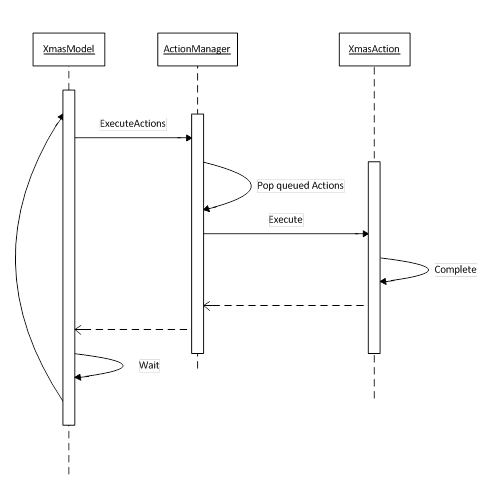
\includegraphics[width=0.7\textwidth]{ImplementationActionQueuingExplanation}
\par\end{centering}

\caption{\label{fig:ImplementationActionQueuingExplanation}A sequence diagram
describing the execution of an action.}
\end{figure}


As can be seen in fig. \ref{fig:ImplementationActionQueuingExplanation}
it starts with the \texttt{XmasModel} running an endless loop that
tells the \texttt{ActionManager} to execute all newly queued actions.
The \texttt{ActionManager} then takes all the actions from a thread
safe list and places them in a local list. After this, each action
is executed individually, putting the action that is being executed
in a running state, this state will not change before the actions
\texttt{Completed} method is called. Once an action has been properly
executed, it will be changed to a completed state and will be properly
disposed of. When the last action has been executed by the \texttt{ActionManager},
the call to \texttt{ExecuteActions} returns and \texttt{XmasModel}
will put the thread in a waiting state. The \texttt{XmasModel} will
remain in a waiting state until a new action has been placed on the
queue; this prevents it from busy waiting when no actions are to be
executed.


\subsubsection*{Considerations}

The way that action completion is designed might seem tedious in that
it has to call the special method \texttt{Completed} on each action.
However it is quite necessary as the completion of the execute method
call does not guarantee that a method is completed, for instance in
the case of non-instantanious actions, as explained in the example
below. 

Consider the action of moving from one place to another. In this case
the move action would need to set a delay before the actual move,
to give the idea that the move action had a speed. As we can\textquoteright{}t
halt other actions during this time it is paramount that the \texttt{Execute}
method is released so that other actions can be executed during this
period. 

This is also how the move action is designed in our reference implementation,
the algorithm is as follows
\begin{enumerate}
\item The move action is put on the queue 
\item The move action sets up a timer on a different thread and finishes
its execution
\item The timer is fired after a given time, and places a new action on
the queue
\item The new action performs the actual move, and calls the \texttt{Completed}
method of its parent Action (the \texttt{MoveAction})
\end{enumerate}
As one can see, the problem in this design is the redundancy created
by having to call the method \texttt{Completed }on every designed
action execution. This might not seem like a problem but it is problematic
in a few ways. First and foremost it adds complexity in usage of the
engine, a person with no knowledge of using the engine would not intuitively
deduce the correct way to make and use actions. Thus it creates a
second problem: there is no way to determine if an action is correctly
constructed during compile time. This means bugs will naturally accumulate
during extended use, even if a user has experience and foreknowledge
forgetting even for a single action can be crucial. This is because
running actions use resources and if never completed the resources
of the actions are never released. For instance let us assume the
\texttt{MoveAction} \texttt{Completed} method is never called, the
result of this is that it is stored in the \texttt{ActionManager}
as \texttt{Running}. Now let us assume that this move action is continuously
being executed by hundreds if not thousands of agents. As each action
is never released the memory stored for each action is never released
and an unintentional memory leak is thus created.

Another way we could have chosen to implement the action completion
process, is the usage of child action. Imagine if an action could
generate new actions that were linked with it, thus the completion
of an action would be tied to the fact that all its child actions
had been executed and not the arbitrary call of a \texttt{Complete}
method. This could undoubtedly provide new problems to overcome and
as such we have not fully followed this path, however given more time
to study the consequences of this design would reveal whether or not
this is a better design. 


\subsubsection*{Summary}

A lot of the considerations when designing the action all comes down
to the reliance on user to clean up the Action, which is generally
not good from a design perspective; it is always preferable that used
data is cleaned up automatically when it is out of scope. However
it is not all bad as this design does guarantee a flexible usage of
the actions; it provides more control to the user which might give
the user abilities to do certain things which would otherwise be denied
within the engine. This is also why this design method was chosen
as our philosophy in the engine design was to minimize limitations
as much as possible while still providing the features we thought
necessary to fulfill the engine's goal.
